\section{Motivations}
\label{sec:motivation}

We focus on computation-heavy ML applications that is beyond the capability of
local devices. In this chapter, we will first show the heterogeneity of swarm
platforms for such heavy computation tasks.

We then motivate profiling by showing the trade-off between application accuracy
and processing times among different algorithms or different parameters for a
given task.

\subsection{Heterogeneous Environment}

\begin{figure}
  \begin{minipage}{0.4\textwidth}
    \centering
    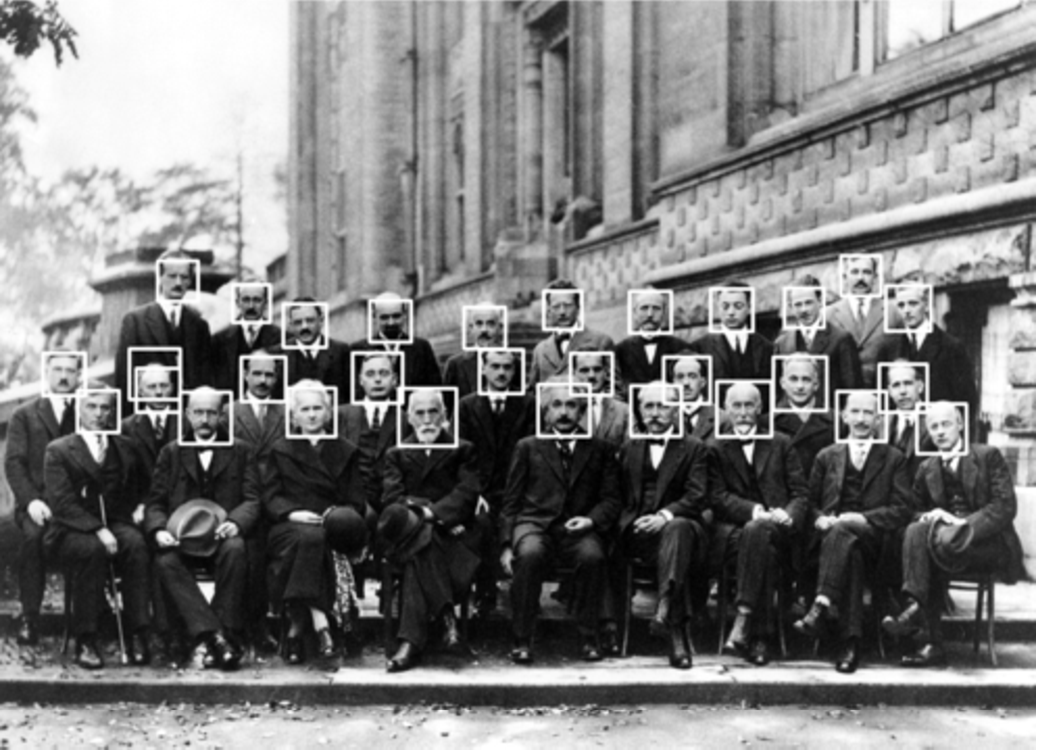
\includegraphics[width=.9\textwidth]{figures/physicist.pdf}
    \label{fig:physicist}
  \end{minipage}%
  \begin{minipage}{0.6\textwidth}
    \centering
    \begin{tabular}{c c c}
      \toprule
      \specialcell{RPi\\Model B}
      & \specialcell{Macbook \\ Model A1502}
      & \specialcell{Workstation\\Xeon E5-1620} \\
      \midrule
      4105 & 544 & 346 \\
      \bottomrule
    \end{tabular}
  \end{minipage}
  \caption{(Left) Face detection with a photograph of the Fifth Solvay
    International Conference on Electrons and Photons. (Right) Processing times
    (ms) on different platforms.}
\end{figure}

Our target application environment consists of machines with large range of
computing resources. $(i)$ End-devices, like mobile phones or IoT platforms, are
significantly limited in their computing power. Performing ML inference often
take seconds to complete. $(ii)$ Edge and Cloud. Both the edge and the cloud
suffers from variable latency, unstable connection, and service contention to
provide consistent response times, especially for 99\% requests.

There is a dizzying array of platforms ranging from \$5 Raspberry Pi to \$1000+
GPU-powered workstation~\cite{zhang2015cloud}.  Even in the cloud, there are
various VM options in the cloud: companies rent VMs based on budget or because
of a lack of expertise.

\subsection{Accuracy-Time Tradeoff}
\label{sec:comp-perf-model}

\begin{figure}
  \centering
  \begin{subfigure}[t]{0.45\textwidth}
    \centering
    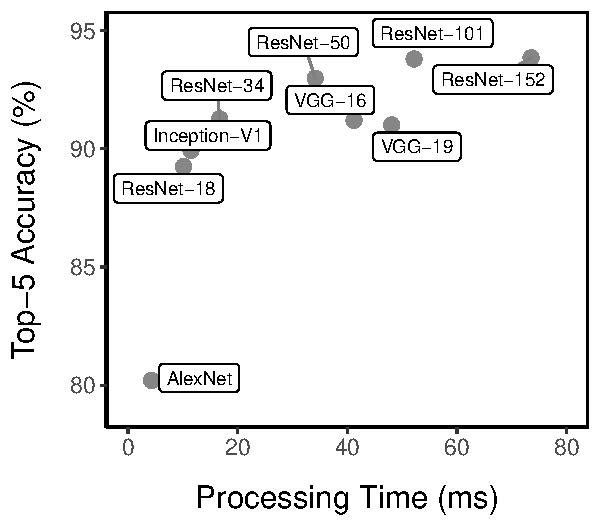
\includegraphics[width=\textwidth]{figures/motiv-functions.pdf}
    \caption{Benchmarks for popular convolutional neural network (CNN) models.}
    \label{fig:motiv-functions}
  \end{subfigure}
  \hfill
  \begin{subfigure}[t]{0.45\textwidth}
    \centering
    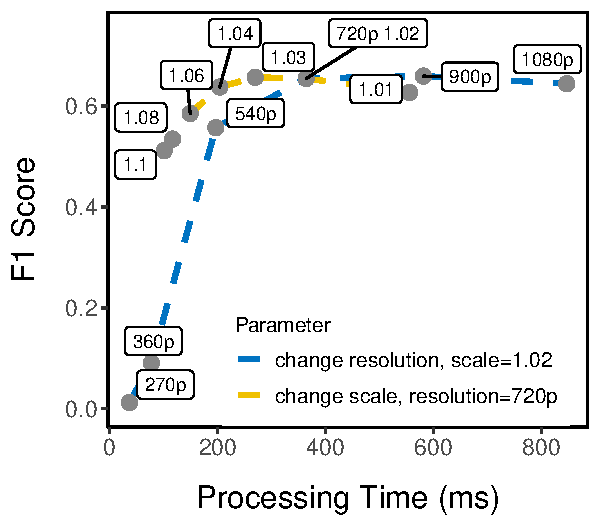
\includegraphics[width=\textwidth]{figures/motiv-params.pdf}
    \caption{Benchmarks for Viola Jones face detection when changing different
      parameters.}
    \label{fig:motiv-params}
  \end{subfigure}
\end{figure}

For many ML inference task, there exist more than one algorithm, or tunable
parameters for each algorithm with different accuracy and processing times.  We
can speed up computation by providing a less accurate response. This would allow
some computation tractable on end devices and handling more requests on the
edge/cloud.

For example, accuracy-cost trade-offs for object detection using convolutional
neural network (CNN)~\cite{huang2016speed}. \autoref{fig:motiv-functions} shows
one such benchmark~\cite{cnn.benchmarks}.

Many algorithms have large number of knobs to tune that will affect accuracy and
processing cost. We use Viola-Jones (VJ) cascade face
detector~\cite{viola2001rapid} as an example. \autoref{fig:complex-perf-model}
shows the large parameter space with respect to three parameters:
\texttt{min\_size}, \texttt{min\_neighbors}, and \texttt{scale}.

ML algorithms have many tunable parameters. For many algorithms, processing
times and the accuracy may exhibit \textit{non-linear} behavior with respect to
the parameters.

\subsection{Challenges}
\label{sec:challenges}

Exhaustive Search is Too Expensive.

\begin{itemize}
\item \texttt{scale}: how much image size is reduced at each image scale.
\item \texttt{min\_size}: minimum detect-able object size.
\item \texttt{min\_neighbors}: how many neighbors each candidate rectangle should
  have to retain it.
\end{itemize}

\begin{figure}[t]
  \centering
  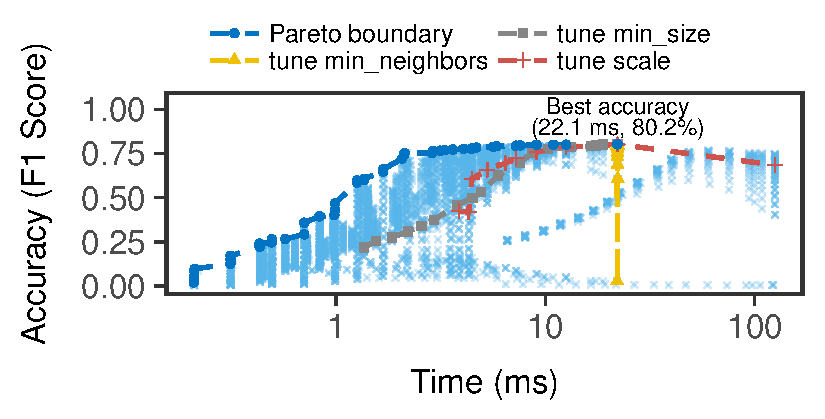
\includegraphics[width=.9\columnwidth]{figures/exhaustive-face.pdf}
  \caption{Complex performance model: spanning multiple dimensions and
    exhibiting non-linear relationship.}
  \label{fig:motiv-params}
\end{figure}

%%% Local Variables:
%%% mode: latex
%%% TeX-master: "../compute"
%%% End:
